\documentclass{article}
\usepackage[utf8]{inputenc}

\title{Rapport projet d'Algorithmique Avancée}
\author{Lydia Rodriguez-de la Nava \& Hakim Baaloudj }
\date{Decembre 2018}

\usepackage{natbib}
\usepackage{graphicx}

\begin{document}

\maketitle

\section{Introduction}
Ce projet s’inscrit dans le cadre de l’UE d’Algorithmique Avancée. Le but de celui-ci est de visualiser graphiquement la complexité en temps d’exécution de structures de données étudiées lors de cette UE : les tas minimum et les files binomiales. 
Nous avons utilisé le langage JAVA pour programmer ce projet.
Pour implémenter les clés de 128bits, nous avons décidé d’utiliser les BigInteger de la librairie JAVA .

Les clés de 128 bits sont stockées dans notre programme comme des BigInteger .

Nous verrons dans un premier temps quels choix nous avons fait pour implémenter nos structures. Nous étudierons les complexités des algorithmes d'union et de construction graphiquement, et nous concluerons sur quelle implémentation de tas est la plus efficace. Enfin, nous effectuerons une étude expérimentale sur l'oeuvre de Shakespeare à l'aide de l'algorithme du MD5 et de nos structures.
\section{Implémentation des structures}

Il nous a été demandé dans un premier temps de coder le tas min sous deux formes : sous forme de tableau, et sous forme d'arbre. Dans un deuxième temps, nous avons dû implémenter une file binomiale. Pour chacune de ces structures, nous allons expliquer leur implémentation dans notre programme.

\subsection{Tas min tableau}

Le tas sous forme de tableau est implémenté avec sa capacité, c’est-à-dire le nombre d ‘élément qu’il peut accueillir, sa taille actuelle et un tableau de clés. Ce dernier est dynamique : à chaque fois que la capacité est atteinte, on double celle-ci.

Pour \textbf{insérer un nouvel élément}, on l’ajoute directement à la fin du tableau puis on lance la fonction percolate\_up() qui va replacer l’élément au bon endroit. Pour faire cela, on compare le nouvel élément avec son père, et si le père est plus petit, on échange les deux éléments, et on recommence jusqu’à ce que l’élément ait un père plus petit que lui, ou bien jusqu’à la racine. On en déduit qu’au pire cas est le cas où l’on doit remonter jusqu’à la racine, donc l’algorithme d’ajout est en $O(\log{}n)$. 

Pour \textbf{supprimer un élément} du tas, on retire le premier élément du tableau et on lance percolate\_down() %A EXPLIQUER il faut préciser la complexité de cet algo

La \textbf{fonction consIter} insère d’abord tous les éléments un à un dans le tableau. Ensuite on appelle percolate\_down sur les éléments, en partant de la fin. %A REMPLIR
De cette façon, au lieu de faire n fois un ajout, ce qui ferait une complexité $O(n\log{}n)$, on se retrouve avec seulement $O(n+m)$.

Pour l'\textbf{union de deux tas}, on crée un nouveau tas vide, puis on lui ajoute avec consIter les éléments du premier tas, puis on rappelle consIter mais cette fois-ci avec les éléments du deuxième tas. On a vu précedemment que consIter était en $O(n)$ or ici on l’appelle sur un tas de taille n et un tas de taille m. On en déduit bien que la complexité est $O(n+m)$.


\subsection{Tas min arbre}
Le tas sous forme d’arbre contient uniquement un pointeur sur le dernier nœud, sachant qu’un nœud contient un élément, un pointeur sur le nœud père, son fils gauche et fils droit.

Pour \textbf{insérer un élément}, on transforme la taille de l’élément en binaire dans un tableau de bits. En fonction de si c’est un 0 ou un 1, on se déplace dans l’arbre (à gauche si c’est un c’est un 0, à droite sinon).

Pour \textbf{supprimer un élément}, on retire tout d’abord la racine %A EXPLIQUER AUSSI

La \textbf{construction par itération}, similairement à la version en arbre, ajoute d’abord tous les éléments un par un, en utilisant la forme binaire pour savoir où placer le nouveau nœud. Puis on appelle  percolate\_down() en partant des derniers pères vers la racine.

Pour l’\textbf{union}, on transforme tous les éléments des deux tas en une liste, puis on lance consInter sur cette liste pour créer un nouveau tas. La création de la liste doit parcourir chaque nœud donc sa complexité est $0(n+m)$ et le constIter d’une liste de taille $n+m$ a une complexité de $O(n+m)$ aussi, donc la complexité est bien $O(n+m)$.


\subsection{File binomiale}

Une file binomiale est implémentée par un tournoi binomial représentant la tête de la file (c'est-à-dire le tournoi au degré maximum), et un tournoi binomial représentant l’arbre avec la racine qui a le plus petit élément de la file. 
Un nœud d’un tournoi binomial contient une référence sur son frère, son fils et son père. De plus, chaque nœud contient un élément et le degré du nœud dans son tournoi.

Les fonctions importantes de la file binomiale utilisent toutes la \textbf{fonction union}. Celle-ci utilise l’algorithme vu en cours qui s’inspire d’une addition entre deux chiffres binaires.

\textbf{Ajouter un élément} dans une file binomiale $FB$ revient à faire une union entre $FB$ et une file binomiale qui ne contient qu'un seul tournoi, qui lui-même ne contient qu'un seul élément. Avant d’ajouter un nouveau tournoi, on compare sa valeur au minimum de la file binomiale pour, si besoin, le modifier. Ainsi, pas besoin de parcourir l’arbre pour retrouver le minimum.

La \textbf{construction par itération} se contente d'appeler itérativement la fonction d'ajout vue juste avant.

Pour \textbf{supprimer le minimum}, on "décapite" le tournoi où se trouve le minimum, c'est-à-dire qu'on transforme ses fils en une file binomiale. D'après la définition d'un tournoi binomial, on peut être sûr que tous les fils de la racine ont un degré différent, et donc on sait que créer une file binomale de ceux-là est correct. On fait ensuite une union avec la file privée du tournoi minimum, et la file créée par décapitation.

\section{Représentation graphique des complexités}

Pour les tests d’union de tas et de files binomiales, nous avons choisi comme stratégie de ranger les fichiers de données en 5 répertoires, un pour chaque jeu. On a ensuite choisi un fichier pivot à 20000 clés auquel on a, pour chaque répertoire, fait union sur tous les fichiers à l’intérieur de chaque répertoire.

Afin d’évaluer le temps d’exécution de chaque fonction, nous avons pris l’heure avant et après le lancement de l’algorithme, puis fait la soustraction. Ceci explique sûrement certaines cassures dans les graphiques. Il aurait été plus précis d’utiliser uniquement le temps passé dans le CPU.

\subsection{Tas min}
\begin{figure}[h!]
\centering
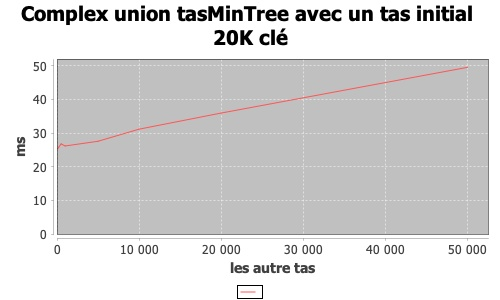
\includegraphics[width=6cm]{tas_tree_union.jpg}\hfill
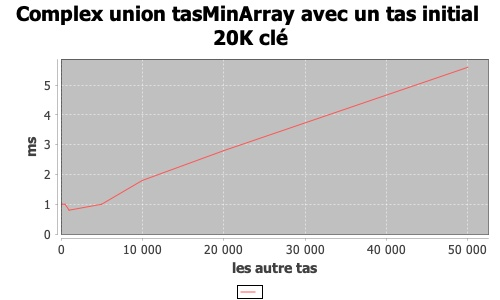
\includegraphics[width=6cm]{tas_array_union.jpg}
\caption{Comparaison complexité de l'algorithme d'union dans un tas min}
\label{fig:tasunion}
\end{figure}


En moyenne, il semble que les complexités pour la version arbre et la version tableau du tas min suivent bien $O(n)$. Cependant, on remarque ici que la version tableau est bien plus rapide que la version arbre. En effet, on voit par exemple que pour $10k$ clés, l’arbre prend 6ms pour s’éxécuter, alors que le tableau n’en prend que $1,5$. De même pour $50k$ clés, l’arbre prend plus de 20ms, alors que le tableau prend 5ms. On en conclut que le tas min implémenté par tableau est en moyenne $3$ fois plus rapide que l’implémentation par arbre dans le cas de construction par itération. 


\begin{figure}[h!]
\centering
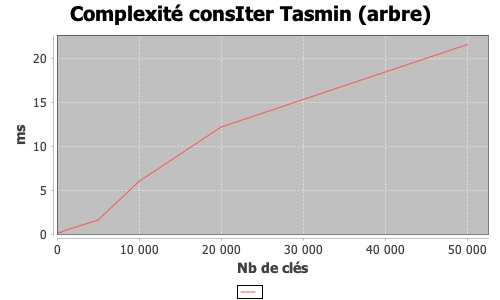
\includegraphics[width=6cm]{tas_tree_consiter.jpg}\hfill
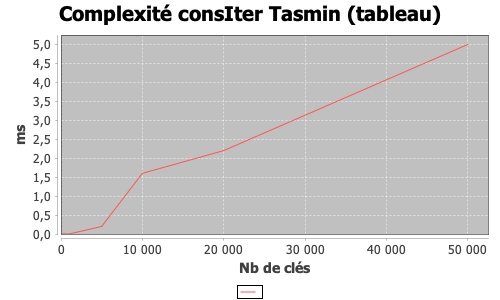
\includegraphics[width=6cm]{tas_array_consiter.jpg}
\caption{Comparaison complexité de l'algorithme consIter dans un tas min}
\label{fig:tasconsiter}
\end{figure}

Pour l’union aussi on semble bien retrouver un temps linéaire pour les deux structures. Ici aussi on remarque que l’implémentation en tableau est bien plus rapide que celle en arbre. Par exemple à $10k$ clés, l’arbre prend un peu plus de $30ms$ alors que que le tableau en met moins de $2ms$. Pour $50k$ clés, on voit bien que le tableau prend $10$ fois moins de temps à effectuer une union.

On en conclut que l’implémentation d’un tas min est plus efficace à l’aide d’une structure utilisant un tableau. Ceci peut s’expliquer par %ARGUMENTER POURQUOI LE TAB EST PLUS RAPIDE

\subsection{File binomiale}


\begin{figure}[h!]
\centering
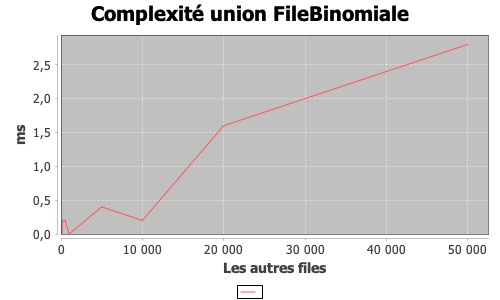
\includegraphics[width=8cm]{fileb_union.jpg}
\caption{Complexité de l'union de deux files binomiales}
\label{fig:fbunio}
\end{figure}



Pour l'union de deux files files, malgré la cassure à $20k$ clés, il semble que le temps est linéaire. Il est possible que cette cassure soit liée à notre stratégie d'étude de la compléxité de l'union puisqu'on va forcément essayer de faire l'union entre le fichier pivot et lui-même dans un des jeux. Or on ne peut pas faire l'union de deux files binomiales avec les mêmes éléments. Ainsi, pour le cas de $20k$ clés, il y avait une union de moins à faire, et donc moins de temps à passer sur ce cas.

\begin{figure}[h!]
\centering
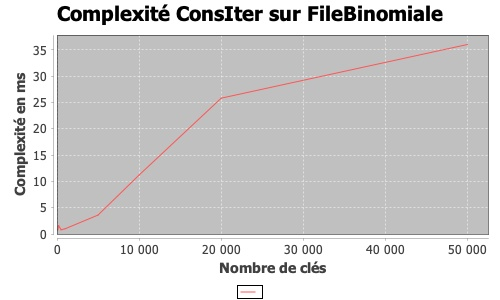
\includegraphics[width=8cm]{FBcomplexConsIter.jpg}
\caption{Complexité de la construction d'une file binomiale}
\label{fig:fbconsi}
\end{figure}

Quant à la construction par itération, le temps d'exécution semble aussi linéaire bien que la construction des files à $20k$ clés ait pris plus de temps que normal.


\section{Etude expérimentale}

Dans cette partie, nous allons étudier graphiquement la différence de temps d'éxécution entre la file binomiale et le tas min. On rappelle qu'on a conclu plus tôt dans ce rapport que l'implémentation du tas min est plus efficace, c'est donc celui-ci que nous avons utilisé pour cette étude.

\subsection{Implémentation de MD5}
Pour transformer un mot en son chiffré MD5, nous avons choisi de transformer en une String de 0 et de 1 la représentation en binaire de 16 bits de chaque caractère. On concatène chaque représentation de caractère dans un autre String, qu’on remplit jusqu’à que sa taille soit un multiple de 512bits, comme décrit dans l’algorithme fournit. La représentation par String est aussi utile pour s’assurer que l’entier est codé en little-endian. Une fois que la String est séparée en 32bits dans le tableau de taille 16, on le retransforme en entier. A la sortie de la grande boucle, on retransforme les 4 entiers en String afin de pouvoir les concaténer en un entier de 128bits et de les traduire en BigInteger ensuite.

Cependant, pour les tests suivants, nous avons dû utiliser le MD5 de la bibliothèque JAVA car notre algorithme ne renvoyait pas la bonne clé. Ceci est peut-être dû au fait que nous n’avons pas utilisé d’entiers non-signé.

\subsection{Comparaison du temps d'éxécution de la file binomiale et du tas min}

Pour les expérimentations suivante, nous avons utilisé un arbre de recherche. % SI TU VEUX DIRE PLUS DE CHOSES A CE SUJET

%je te laisse expliquer comment tu as construit l’arbre de recherche et la liste et répondre à 6.13


Pour les graphiques suivants, on peut voir à l’abscisse de valeur 50 le temps qu’a mis le tas min et à 100  le temps qu’a mis la file binomiale à effectuer l’algorithme.

\subsubsection{Ajout d'un élément}

Pour étudier la complexité de l'ajout, on a ajouté chaque mot distinct un à un dans chaque structure.

\begin{figure}[h!]
\centering
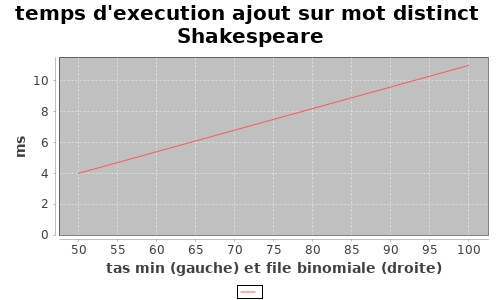
\includegraphics[width=8cm]{ajout_SP_tas_array.jpg}
\caption{Complexité en temps de l'ajout}
\label{fig:fbtasajout}
\end{figure}

On voit que la file binomiale est 2,5 fois plus lente que le tas pour cet algorithme . Ceci s’explique notamment par le fait que %si tu as de l'inspiration

\subsubsection{Suppression de l'élément minimum}

Pour la suppression, on a repris les structures construites juste avant avec l'ajout, puis on a supprimé chaque minimum un par un jusqu'à ce que les structures soient vides.

\begin{figure}[h!]
\centering
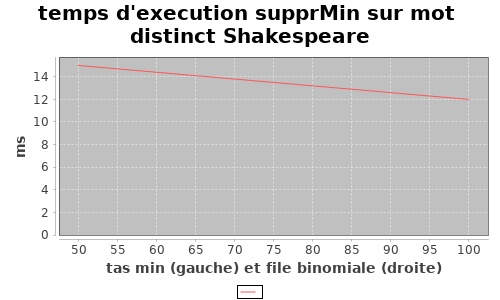
\includegraphics[width=8cm]{supprmin_SP_tas_array.jpg}
\caption{Complexité en temps de la suppression de min}
\label{fig:fbtassuppr}
\end{figure}

On regarde maintenant la complexité pour supprimer tous les éléments ds structures construites précédemment par ajouts consécutifs, par ordre croissant. On remarque ici que le tas met environ 2,5ms de plus à se vider que la file binomiale. %pareil si tu as de l'inspi pour justifier

\subsubsection{Construction par itération}

Pour la construction, on a reconstruit entièrement chaque structure avec chaque mot distinct.

\begin{figure}[h!]
\centering
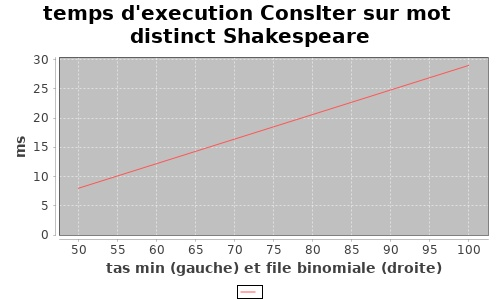
\includegraphics[width=8cm]{consiter_SP_tas_array.jpg}
\caption{Complexité en temps de la suppression de min}
\label{fig:fbtascons}
\end{figure}

Pour cet algorithme-ci, le tas est bien plus efficace que la file binomiale. En effet, le tas est 4 fois plus rapide pour se construire. %toujours pas inspirée pour justifier

\subsubsection{Union de deux structures}

Pour l’union, notre stratégie a été de créer pour chaque structure deux instances chacune une moitié de la liste de mots, et d’ensuite les unir en une seule. 
\begin{figure}[h!]
\centering
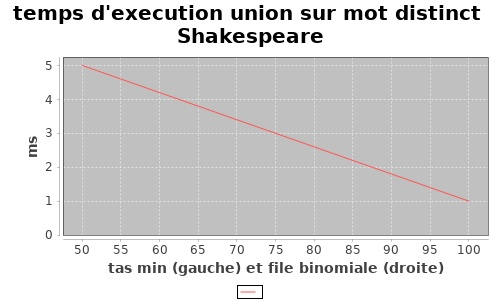
\includegraphics[width=8cm]{union_SP_tas_array.jpg}
\caption{Complexité en temps de la suppression de min}
\label{fig:fbtascons}
\end{figure}

On remarque ici que la file binomiale est 5 fois plus rapide pour effectuer une union que le tas. Ceci s’explique notamment par le fait que l’union de deux files binomiales consiste en uniquement comparer les tournois de même taille et d’ajouter un lien dans ce cas, alors qu’un tas doit ajouter tous les éléments des deux structures à unir puis parcourir la moitié de ces éléments pour vérifier qu’elles respectent les règles d’un tas min. La file binomiale a donc bien moins de travail à effectuer.

\section{Conclusion}
On peut déduire de ces expérimentations que pour la construction, le tas min est bien plus efficace que la file binomiale. Cependant, pour supprimer le minimum ou unir deux structures, c’est la file binomiale qui est la plus efficace. De ce fait, il est difficile de conclure sur quelle structure est plus efficace, cela dépend de l’utilisation qu’on compte faire de la structure. De manière générale, si le but est de stocker beaucoup de valeurs, il vaut mieux utiliser un tas min. Cependant, si l’on a prévu de faire beaucoup d’opérations comme l’union ou la suppression, peut-être est-il plus avantageux de choisir une file binomiale.



\section{Reférences}

Thomas H. Cormen, Charles E. Leiserson, Ronald L. Rivest et Clifford Stein,\textit{ Introduction à l'Algorithmique}, Paris, Dunod, 2010, 3e éd.

Pour le MD5 : https://en.wikipedia.org/wiki/MD5
\end{document}
